\documentclass[12pt,a4paper]{article}
\usepackage{charter}
%\usepackage[latin1]{inputenc}
\usepackage[left=1.50cm, right=1.50cm, top=1.20cm]{geometry}
\usepackage{amsmath}
\usepackage{amsfonts}
\usepackage{amssymb}
\usepackage{graphicx}
\usepackage{textcomp}
\renewcommand{\baselinestretch}{1.5}
\usepackage{listings}
\usepackage{xcolor}
\definecolor{listinggray}{gray}{0.9}
\definecolor{lbcolor}{rgb}{0.9,0.9,0.9}
\usepackage{float}
\usepackage{CJKutf8}
\usepackage{textcomp}
\usepackage{hyperref}
%\lstset{
%	backgroundcolor=\color{lbcolor},
%	tabsize=4,    
%	%   rulecolor=,
%	language=[GNU]C++,
%	basicstyle=\scriptsize,
%	upquote=true,
%	aboveskip={1.5\baselineskip},
%	columns=fixed,
%	showstringspaces=false,
%	extendedchars=false,
%	breaklines=true,
%	prebreak = \raisebox{0ex}[0ex][0ex]{\ensuremath{\hookleftarrow}},
%	frame=single,
%	numbers=left,
%	showtabs=false,
%	showspaces=false,
%	showstringspaces=false,
%	identifierstyle=\ttfamily,
%	keywordstyle=\color[rgb]{0,0,1},
%	commentstyle=\color[rgb]{0.026,0.112,0.095},
%	stringstyle=\color[rgb]{0.627,0.126,0.941},
%	numberstyle=\color[rgb]{0.205, 0.142, 0.73},
%	%        \lstdefinestyle{C++}{language=C++,style=numbers}?.
%}
%\lstset{
%	backgroundcolor=\color{lbcolor},
%	tabsize=4,
%	language=C++,
%	captionpos=b,
%	tabsize=3,
%	frame=lines,
%	numbers=left,
%	numberstyle=\tiny,
%	numbersep=5pt,
%	breaklines=true,
%	showstringspaces=false,
%	basicstyle=\footnotesize,
%	%  identifierstyle=\color{magenta},
%	keywordstyle=\color[rgb]{0,0,1},
%	commentstyle=\color{Darkgreen},
%	stringstyle=\color{red}
%}

\lstdefinestyle{customc}{
	belowcaptionskip=1\baselineskip,
	aboveskip={1.2\baselineskip},
	breaklines=true,
	frame=lines,
	numbers=left,
	xleftmargin=\parindent,
	language=C++,
	showstringspaces=false,
	basicstyle=\sffamily,%,\ttfamily,
	keywordstyle=\bfseries\color{green!40!black},
	commentstyle=\itshape\color{purple!40!black},
	identifierstyle=\color{blue},
	stringstyle=\color{orange},
	breaklines=true,
	postbreak=\raisebox{0ex}[0ex][0ex]{\ensuremath{\color{red}\hookrightarrow\space}}
}

\lstdefinestyle{customasm}{
	belowcaptionskip=1\baselineskip,
	frame=L,
	xleftmargin=\parindent,
	language=[x86masm]Assembler,
	basicstyle=\footnotesize\ttfamily,
	commentstyle=\itshape\color{purple!40!black},
}

\lstset{escapechar=@,style=customc}

\begin{document}
\section{80}
\begin{CJK}{UTF8}{gbsn}
这道题是之前那道 Remove Duplicates from Sorted Array 有序数组中去除重复项 的延续,这里允许最多重复的次数是两次,那么我们就需要用一个变量count来记录还允许有几次重复,count初始化为1,如果出现过一次重复,则count递减1,那么下次再出现重复,快指针直接前进一步,如果这时候不是重复的,则count恢复1,由于整个数组是有序的,所以一旦出现不重复的数,则一定比这个数大,此数之后不会再有重复项
\end{CJK}
\begin{lstlisting}
int removeDuplicates(int A[], int n) {
	if (n <= 2) return n;
	int pre = 0, cur = 1, count = 1;
	while (cur < n) {
		if (A[pre] == A[cur] && count == 0) ++cur;
		else {
			if (A[pre] == A[cur]) --count;
			else count = 1;
			A[++pre] = A[cur++];
		}
	}
	return pre + 1;
}
\end{lstlisting}

\section{81}
\begin{CJK}{UTF8}{gbsn}
这道是之前那道 Search in Rotated Sorted Array 在旋转有序数组中搜索 的延伸,现在数组中允许出现重复数字,这个也会影响我们选择哪半边继续搜索,由于之前那道题不存在相同值,我们在比较中间值和最右值时就完全符合之前所说的规律:如果中间的数小于最右边的数,则右半段是有序的,若中间数大于最右边数,则左半段是有序的。而如果可以有重复值,就会出现来面两种情况,[3 1 1] 和 [1 1 3 1],对于这两种情况中间值等于最右值时,目标值3既可以在左边又可以在右边,那怎么办么,对于这种情况其实处理非常简单,只要把最右值向左一位即可继续循环,如果还相同则继续移,直到移到不同值为止,然后其他部分还采用 Search in Rotated Sorted Array 在旋转有序数组中搜索 中的方法
\end{CJK}
\begin{lstlisting}
bool search(int A[], int n, int target) {
	if (n == 0) return false;
	int left = 0, right = n - 1;
	while (left <= right) {
		int mid = (left + right) / 2;
		if (A[mid] == target) return true;
		else if (A[mid] < A[right]) {
			if (A[mid] < target && A[right] >= target) left = mid + 1;
			else right = mid - 1;
		}
		else if (A[mid] > A[right]) {
			if (A[left] <= target && A[mid] > target) right = mid - 1;
			else left = mid + 1;
		}
		else --right;
	}
	return false;
}
\end{lstlisting}


\section{82}
\begin{CJK}{UTF8}{gbsn}
这里要删掉所有的重复项,由于链表开头可能会有重复项,被删掉的话头指针会改变,而最终却还需要返回链表的头指针。所以需要定义一个新的节点,然后链上原链表,然后定义一个前驱指针和一个现指针,每当前驱指针指向新建的节点,现指针从下一个位置开始往下遍历,遇到相同的则继续往下,直到遇到不同项时,把前驱指针的next指向下面那个不同的元素。如果现指针遍历的第一个元素就不相同,则把前驱指针向下移一位
\end{CJK}
\begin{lstlisting}
ListNode *deleteDuplicates(ListNode *head) {
	if (!head || !head->next) return head;

	ListNode *start = new ListNode(0);
	start->next = head;
	ListNode *pre = start;
	while (pre->next) {
		ListNode *cur = pre->next;
		while (cur->next && cur->next->val == cur->val) cur = cur->next;
		if (cur != pre->next) pre->next = cur->next;
		else pre = pre->next;
	}
	return start->next;
}
\end{lstlisting}

\section{83}
\begin{CJK}{UTF8}{gbsn}
移除有序链表中的重复项需要定义个指针指向该链表的第一个元素,然后第一个元素和第二个元素比较,如果重复了,则删掉第二个元素,如果不重复,指针指向第二个元素。这样遍历完整个链表,则剩下的元素没有重复项。
\end{CJK}
\begin{lstlisting}
ListNode *deleteDuplicates(ListNode *head) {
	if (!head || !head->next) return head;

	ListNode *start = head;
	while (start && start->next) {
		if (start->val == start->next->val) {
			ListNode *tmp = start->next;
			start->next = start->next->next;
			delete tmp;
		}
		else start = start->next;
	}
	return head;
}
\end{lstlisting}

\section{84}
\begin{CJK}{UTF8}{gbsn}
维护一个栈,用来保存递增序列,相当于上面那种方法的找局部峰值,当当前值小于栈顶值时,取出栈顶元素,然后计算当前矩形面积,然后再对比当前值和新的栈顶值大小,若还是栈顶值大,则再取出栈顶,算此时共同矩形区域面积,照此类推,可得最大矩形。通过题目中的[2,1,5,6,2,3]作为例子看看
\\
首先,如果栈是空的,那么索引$i$入栈。那么第一个$i=0$就进去吧。注意栈内保存的是索引,不是高度。然后i++
\end{CJK}
\begin{center}
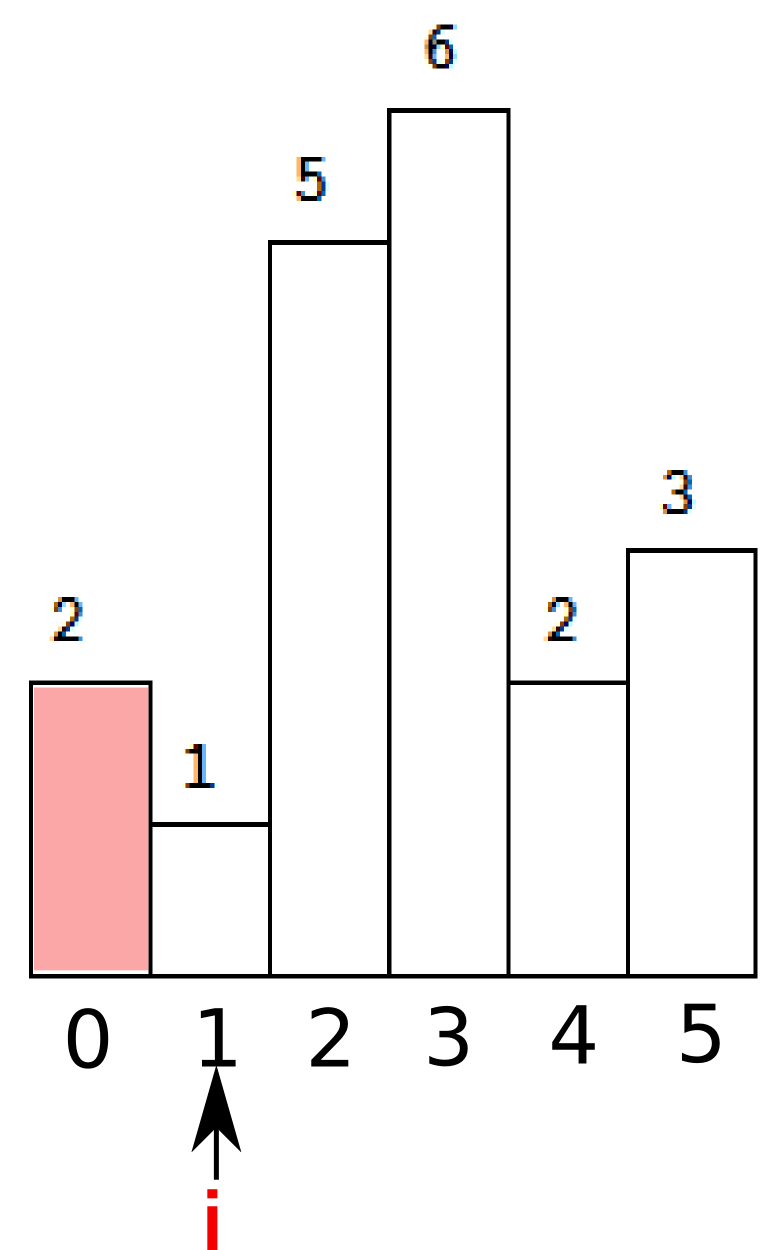
\includegraphics[width=0.5\linewidth]{008401.png}
\end{center}
\begin{CJK}{UTF8}{gbsn}
然后继续,当$i=1$的时候,发现$h[i]$小于了栈内的元素,于是出栈。(由此可以想到,哦,看来stack里面只存放单调递增的索引)
这时候stack为空,所以面积的计算是$h[t] \times i$. $t$是刚刚弹出的stack顶元素。也就是蓝色部分的面积。
\end{CJK}
\begin{center}
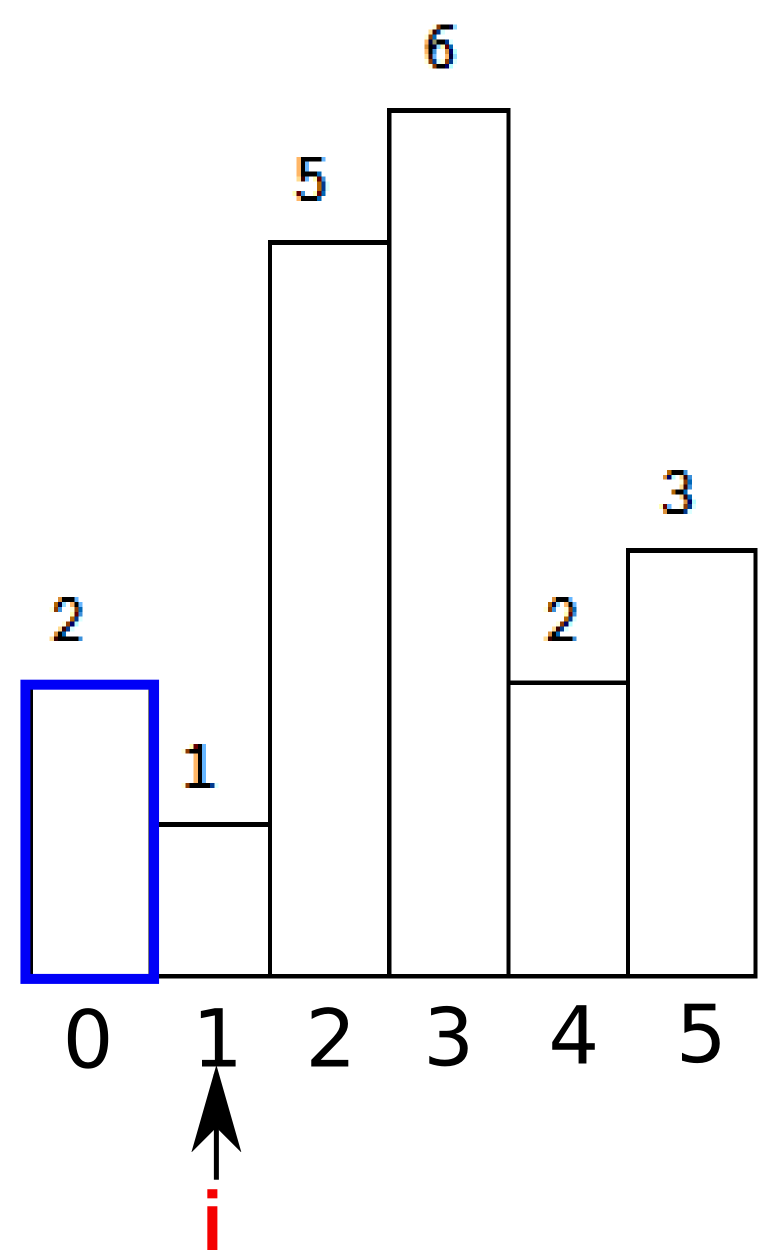
\includegraphics[width=0.5\linewidth]{008402.png}
\end{center}
\begin{CJK}{UTF8}{gbsn}
继续。这时候stack为空了,继续入栈。注意到只要是连续递增的序列,我们都要keep pushing,直到我们遇到了$i=4$,$h[i]=2$小于了栈顶的元素。
\end{CJK}
\begin{center}
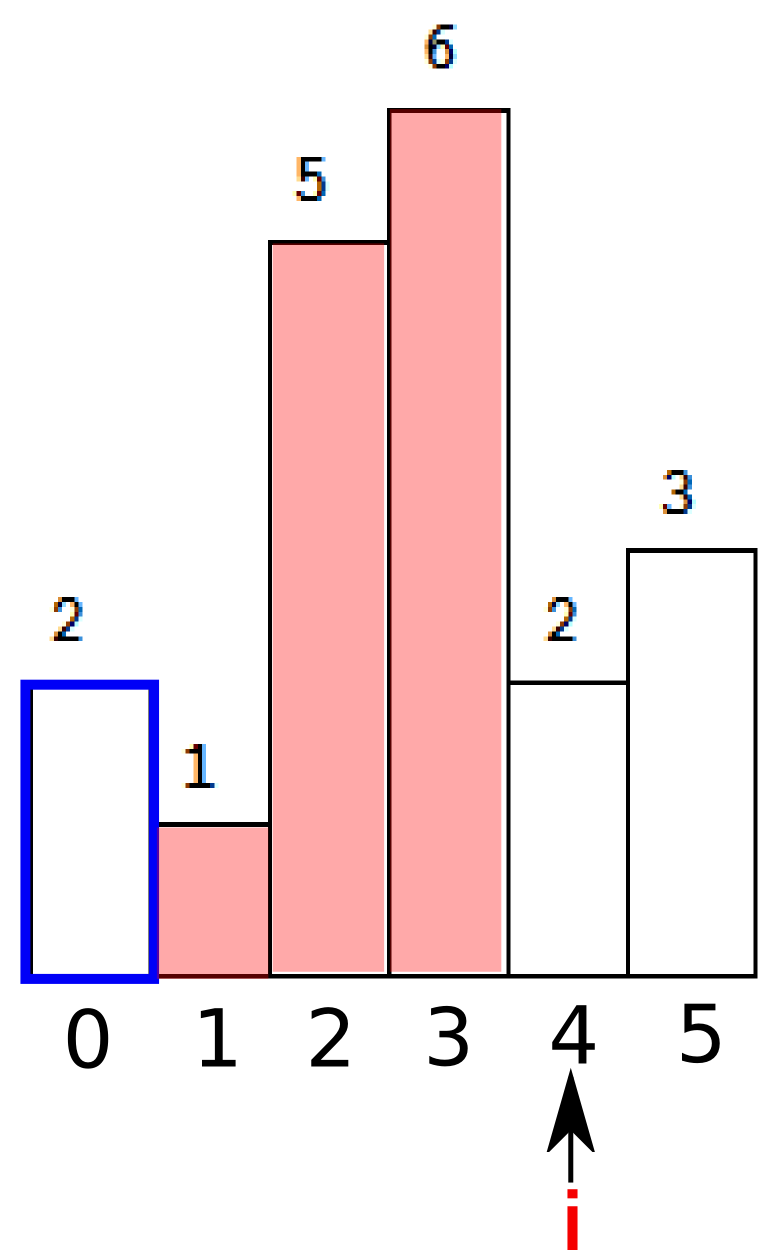
\includegraphics[width=0.5\linewidth]{008403.png}
\end{center}
\begin{CJK}{UTF8}{gbsn}
这时候开始计算矩形面积。首先弹出栈顶元素,$t=3$。即下图绿色部分。
\end{CJK}
\begin{center}
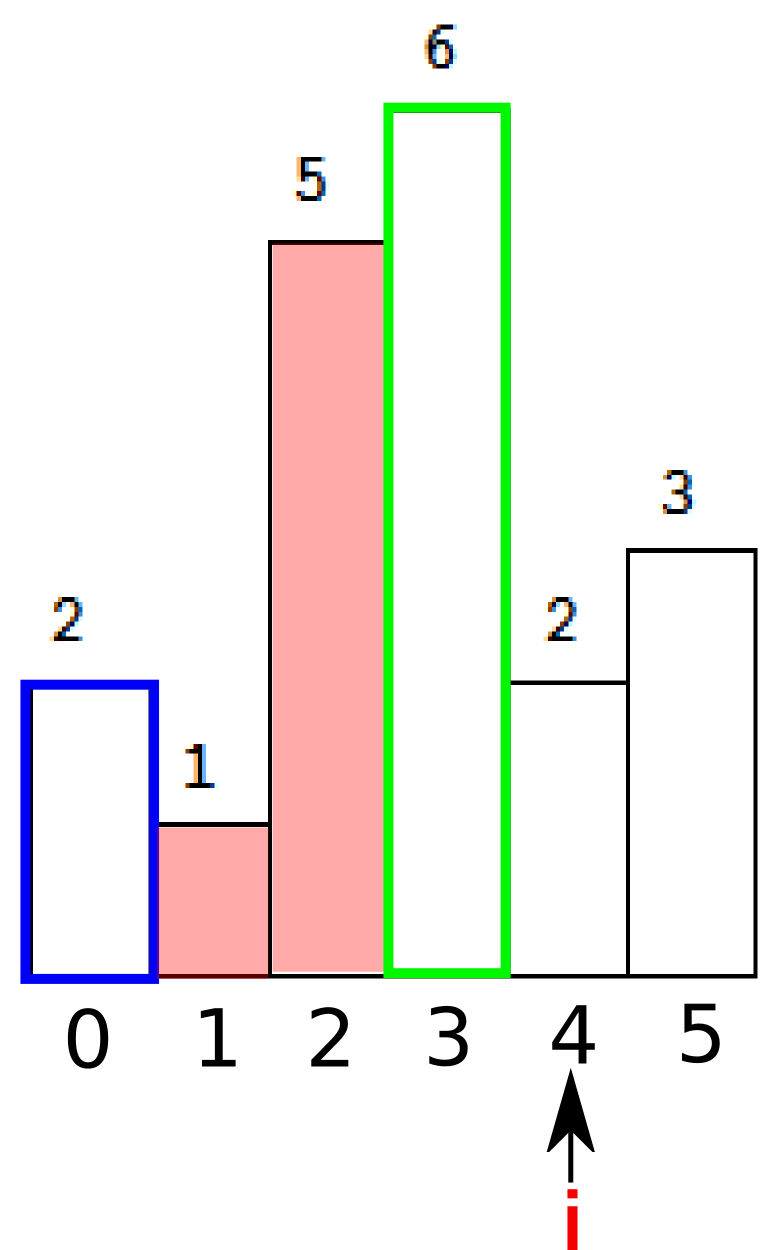
\includegraphics[width=0.5\linewidth]{008404.png}
\end{center}
\begin{CJK}{UTF8}{gbsn}
接下来注意到栈顶的(索引指向的)元素还是大于当前i指向的元素,于是出栈,并继续计算面积,桃红色部分。
\end{CJK}
\begin{center}
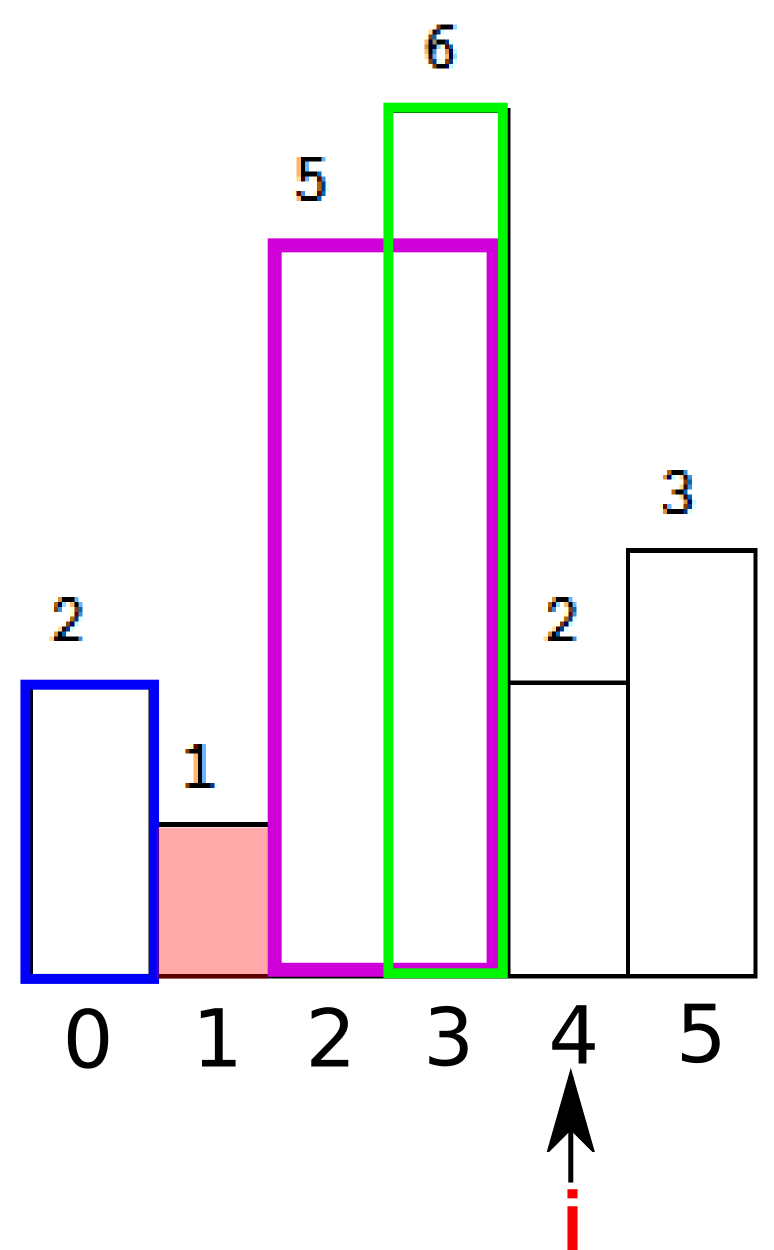
\includegraphics[width=0.5\linewidth]{008405.png}
\end{center}
\begin{CJK}{UTF8}{gbsn}
最后,栈顶的(索引指向的)元素大于了当前$i$指向的元素,循环继续,入栈并推动$i$前进。直到我们再次遇到下降的元素,也就是我们最后人为添加的dummy元素0.
\end{CJK}
\begin{center}
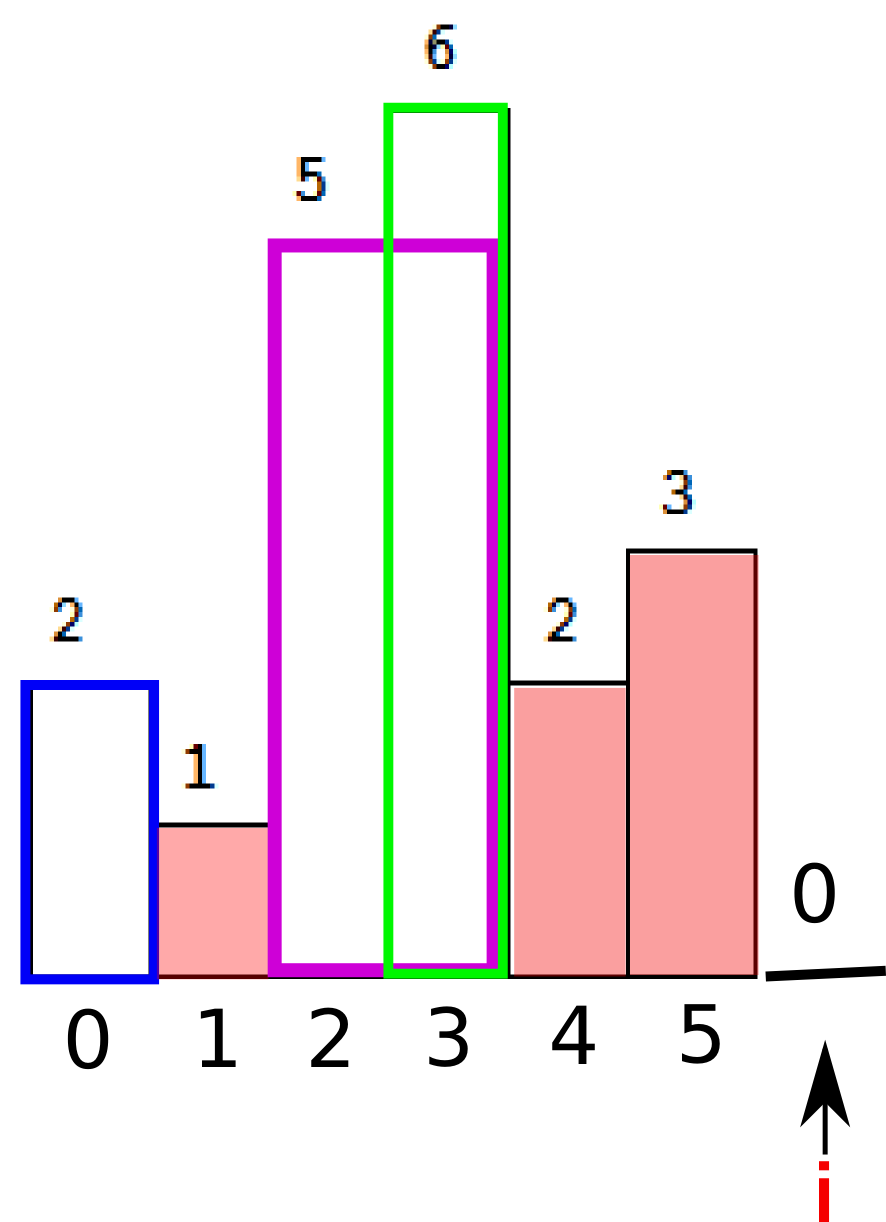
\includegraphics[width=0.5\linewidth]{008406.png}
\end{center}
\begin{CJK}{UTF8}{gbsn}
同理,我们计算栈内的面积。由于当前$i$是最小元素,所以所有的栈内元素都要被弹出并参与面积计算。
\end{CJK}
\begin{center}
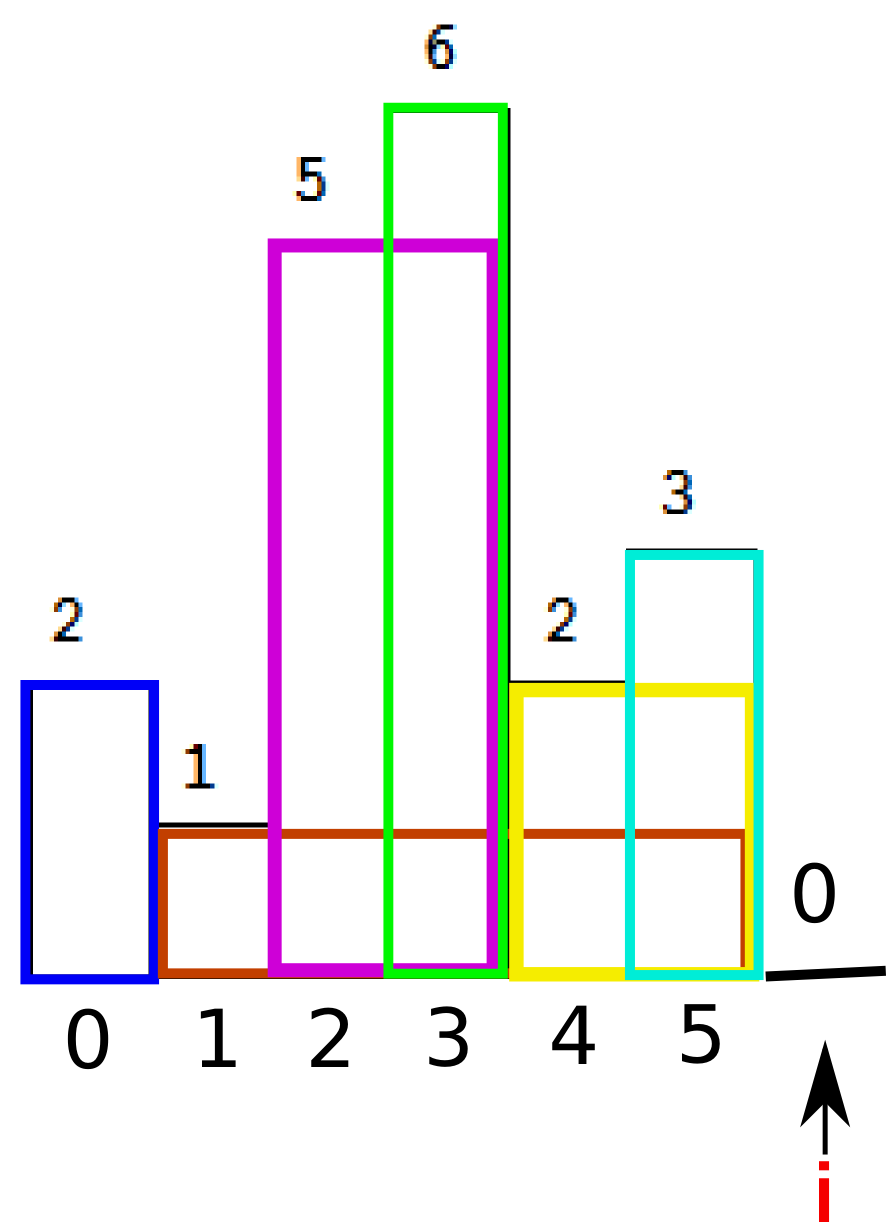
\includegraphics[width=0.5\linewidth]{008407.png}
\end{center}
\begin{CJK}{UTF8}{gbsn}
注意我们在计算面积的时候已经更新过了maxArea。总结下,我们可以看到,stack中总是保持递增的元素的索引,然后当遇到较小的元素后,依次出栈并计算栈中bar能围成的面积,直到栈中元素小于当前元素。
\end{CJK}
\begin{lstlisting}
int largestRectangleArea(vector<int> &height) {
	int res = 0;
	stack<int> s;
	height.push_back(0);
	for (int i = 0; i < height.size(); ++i) {
		if (s.empty() || height[s.top()] < height[i]) s.push(i);
		else {
			int cur = s.top();
			s.pop();
			res = max(res, height[cur] * (s.empty() ? i : (i - s.top() - 1)));
			--i;
		}
	}
	return res;
}
\end{lstlisting}


\section{75}
\begin{CJK}{UTF8}{gbsn}
\end{CJK}
\begin{lstlisting}
\end{lstlisting}

\section{76}
\begin{CJK}{UTF8}{gbsn}\end{CJK}
\begin{lstlisting}
\end{lstlisting}

\section{77}
\begin{CJK}{UTF8}{gbsn}
\end{CJK}
\begin{lstlisting}
\end{lstlisting}

\section{78}
\begin{CJK}{UTF8}{gbsn}
\end{CJK}
\begin{lstlisting}
\end{lstlisting}

\section{79}
\begin{CJK}{UTF8}{gbsn}
\end{CJK}
\begin{lstlisting}
\end{lstlisting}
\end{document}